\chapter{Développement Android}
\section{Android en bref}
Java, activity, fragment, services, permissions

\bigskip
\begin{img}
  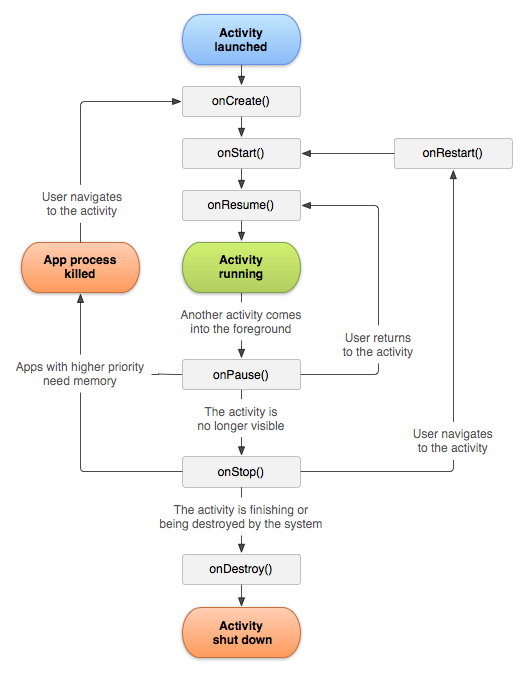
\includegraphics[scale=0.5]{img/cycle.png}
  \caption{Cycle de vie d'une Activity}
\end{img}


\section{Structure du projet}
\bigskip
\begin{multicols}{2}
\begin{img}
  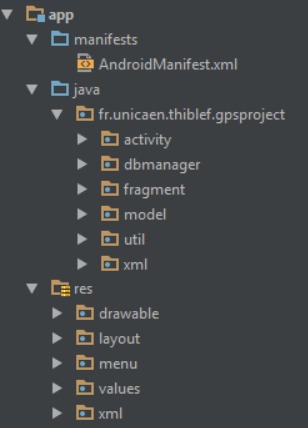
\includegraphics[scale=0.5]{img/archi.png}
  \caption{Structure de l'application}
\end{img}

\end{multicols}

\section{Fonctionnement des layouts}
\begin{xml}[Exemple d'un layout]
<?xml version="1.0" encoding="utf-8"?>
<LinearLayout xmlns:android="http://schemas.android.com/apk/res/android"
    android:orientation="vertical" android:layout_width="match_parent"
    android:layout_height="match_parent">	
	<TextView
    	android:layout_width="match_parent"
        android:layout_height="match_parent"
        android:id="@+id/textView"
        android:layout_weight="0.5"
        android:text="@string/temps" />
                
    <fragment
        android:id="@+id/map_container"
        android:layout_width="fill_parent"
        android:layout_height="fill_parent"
        android:layout_weight="0.5"
        class="com.google.android.gms.maps.SupportMapFragment"
        android:name="com.google.android.gms.maps.SupportMapFragment" />
</LinearLayout>
\end{xml}
\section{}


